\documentclass{beamer}                             % presentation
% \documentclass[draft]{beamer}                    % improves compile time
% \documentclass[11pt, handout]{beamer}            % handout
\usepackage[utf8]{inputenc}                        % utf8
\usepackage[T1]{fontenc}                           % fix font encoding
\usepackage[english]{babel}                        % language
\usepackage{geometry, hyperref, fancyhdr, algorithm}
\usepackage{amsmath, amssymb, amsthm}              % ams mathematical packages
\usepackage{physics, mathtools, bm}                % extra math packages
\usepackage{graphicx, subcaption, wrapfig}         % images
\usepackage{fvextra, textcomp, CJKutf8}            % misc. text formatting
\usepackage[autostyle, english=american]{csquotes} % quotes
\usepackage{tikz, pgfplots, tikz-network}          % plots and graphs
\usepackage[noend]{algpseudocode}                  % algorithm psuedocode
\usepackage[cache=true]{minted}                    % source code
\usepackage[style=ieee]{biblatex}                  % bibliography

\pgfplotsset{compat=1.17}                          % version of pgfplots

\hypersetup{
  colorlinks=true,
  urlcolor=cyan,
  linkcolor=magenta
}

\setminted[]{
  linenos=false,
  breaklines=true,
  encoding=utf8,
  fontsize=\normalsize,
  frame=lines,
  framesep=2mm
}

% https://tex.stackexchange.com/questions/343494/minted-red-box-around-greek-characters
\makeatletter
\AtBeginEnvironment{minted}{\dontdofcolorbox}
\def\dontdofcolorbox{\renewcommand\fcolorbox[4][]{##4}}
\makeatother

\graphicspath{{./images/}}
\addbibresource{ref.bib}

\newcommand{\emphasis}[1]{\textbf{\textit{#1}}}
\DeclareMathOperator{\E}{E}
\DeclareMathOperator{\Var}{Var}

\usetheme{Berkeley}
\usecolortheme{dolphin}
% hide navigation buttons
\setbeamertemplate{navigation symbols}{}

% title page
\title[]{Otsu's Binarization}
\subtitle{}
\author[Huan]{Stephen Huan\inst{1}}
\institute[TJHSST]
{
  \inst{1}
  Thomas Jefferson High School for Science and Technology
}
\date[]{TJ Vision \& Graphics Club, April 14, 2021}
\subject{Computer Science}

\AtBeginSubsection[]
{
  \begin{frame}
    \frametitle{Table of Contents}
    \tableofcontents[currentsection, currentsubsection]
  \end{frame}
}

\begin{document}
\frame{\titlepage}

\section{Probability Theory}

\begin{frame}
\frametitle{Probability Theory}
\framesubtitle{}
Before we start, we'll need to know some basic probability...
\end{frame}

\subsection{Definition}

\begin{frame}
\frametitle{Basic Definitions}
\framesubtitle{}

\begin{definition}
  The \textit{sample space} is the set of all possible outcomes, commonly
  denoted \( \Omega \). An \textit{event} is just \enquote{something which
  occurs}, or formally speaking, a set which is a subset of \( \Omega \).
\end{definition}

\begin{definition}
  The \textit{class of events} \( \mathcal{F} \) is a \( \sigma \)-algebra
  on \( \Omega \) (that is, it is a collection of the subsets of \( \Omega
  \), including \( \Omega \), and closed under union and complement). We
  will assume \( \mathcal{F} = \mathcal{P}(\Omega) \), the power set of \(
  \Omega \) (the set of all subsets of \( \Omega \)).
\end{definition}

\end{frame}

\begin{frame}
\frametitle{Probability Function}
\framesubtitle{}
\begin{definition}
  (Kolmogorov axioms) Given a sample space \( \Omega \) and event class \(
  \mathcal{F} \), a probability function \( P \) has the following properties:
  \begin{enumerate}
    \item \( P(E) \in \mathbb{R}, P(E) \geq 0 \) for all \( E \in \mathcal{F} \) 
    \item \( P(\Omega) = 1 \)
    \item If \( E_1 \) and \( E_2 \) are disjoint sets in \( \mathcal{F} \),
      \( P(E_1 \cup E_2) = P(E_1) + P(E_2) \)
  \end{enumerate}
  It follows that \( (\Omega, \mathcal{F}, P) \)
  is a \textit{probability space}.
\end{definition} 
\end{frame}

\begin{frame}
\frametitle{Law of Total Probability}
\framesubtitle{}
\begin{theorem}
  If \( B_i \) is a partition of \( \Omega \), then
  \( P(A) = \sum_i P(A \cap B_i) \)
\end{theorem}
\begin{proof}
  Let's look at the sum of the first two terms. 
  \( P(A \cap B_1) + P(A \cap B_2) = P((A \cap B_1) \cup (A \cap B_2)) \) 
  because \( A \cap B_1 \) and \( A \cap B_2 \) are
  disjoint (\( B_1 \) and \( B_2 \) are disjoint).
  \( = P(A \cap (B_1 \cup B_2)) \).
  Extending the logic to all \( B_i \),
  \[ = P(A \cap (B_1 \cup B_2 \cup \dots \cup B_n)) \]
  We know \( B_1 \cup B_2 \cup \dots \cup B_n = \Omega \) since
  it's a partition, and \( A \cap \Omega = A \) by definition.
  So this is just \( P(A) \).
\end{proof}
\end{frame}

\subsection{Expectation and Variance}

\begin{frame}
\frametitle{Random Variable}
\framesubtitle{}
\begin{definition} 
  A \textit{random variable} (r.v.) is a function \( \Omega \to \mathbb{R} \),
  i.e. a function assigning a number to each outcome, but can more intuitively
  be thought of as a \enquote{dispenser} of values. We will denote random
  variables as a single uppercase letter, e.g. \( X \) or \( Z \).
\end{definition}
\begin{alertblock}{Randomness}
  Although the probability space carries \enquote{randomness}, a random
  variable is neither random nor a variable --- it is a deterministic function
  assigning a fixed number to a particular outcome. Although what outcome you
  get is random (from the randomness of the space), the assignment is the same.
\end{alertblock}
\end{frame}

\begin{frame}
\frametitle{Expected Value}
\framesubtitle{}
\begin{definition}
  The \textit{expected value} is what we \enquote{expect} a random variable to
  dispense over many samples, or the average value: 
  \[ \E[X] = \sum_{x \in X} x \, P(x) \] 
  We will also denoted the expected value as \( \mu \).
\end{definition}
\begin{exampleblock}{Example}
  Let \( X \) take on value 1 with probability \( \frac{1}{2} \), 2 with
  \( \frac{1}{4} \) chance, and 3 with \( \frac{1}{4} \) chance.
  \( \E[X] = 2 \cdot \frac{1}{2} + 2 \cdot \frac{1}{4} + 3 \cdot \frac{1}{4} 
           = \frac{9}{4} \).
\end{exampleblock}
\end{frame}

\begin{frame}
\frametitle{Law of the Unconscious Statistician}
\framesubtitle{}
\begin{theorem}
  \( \E[f(X)] = \sum_{x \in X} f(x) \, P(x) \), i.e. the expected value of a
  transformation of a random variable.
\end{theorem}
\begin{proof}
  (informal) We can think of \( f(x) \) as partitioning \( X \) into
  subsets like \( S = \{ x \in X \mid f(x) = y \} \) for some \( y \).
  When we compute \( P(y) \), it'll be the sum of \( P(x) \) for all
  \( x \in S \). But we know each \( S(y) \) is disjoint for different
  values of \( y \) since they necessarily form a partition. So if we
  iterate over \( x \), we cover the same set anyways, multiplying each
  \( P(x) \) by the \( f(x) \) it belongs to.
\end{proof}
\end{frame}

\begin{frame}
\frametitle{Linearity of Expectation}
\framesubtitle{}
\begin{corollary}
  The linearity of expectation, i.e.
  \begin{enumerate}
    \item \( \E[X + Y] = \E[X] + \E[Y] \) for random variables \(X, Y\) 
    \item \( \E[cX] = c\E[X] \) for \( c \in \mathbb{R} \)
  \end{enumerate}
\end{corollary}
\end{frame}

\begin{frame}
\frametitle{Proof of Linearity of Expectation}
\framesubtitle{}
\begin{proof}
  Begin with the definition of expectation:
  \begin{align*}  
    \E[X + Y] &= \sum_{x \in X} \sum_{y \in Y} (x + y) \, P(x, y) \\
              &= \sum_{x \in X} \sum_{y \in Y} x \, P(x, y) +
                 \sum_{x \in X} \sum_{y \in Y} y \, P(x, y) \\
    \shortintertext{Swapping order and applying the law of total probabilities,}
              &= \sum_{x \in X} x \underbrace{\sum_{y \in Y} P(x, y)}_{P(x)} + 
                 \sum_{y \in Y} y \underbrace{\sum_{x \in X} P(x, y)}_{P(y)} \\
              &= \sum_{x \in X} x \, P(x) + \sum_{y \in Y} y \, P(y)
               = \E[X] + \E[Y]
  \end{align*}
  \let\qedsymbol\relax
\end{proof}
\end{frame}

\begin{frame}
\frametitle{Proof of the Linearity of Expectation, Continued}
\framesubtitle{}
\begin{proof}
  We use the transformation \( f(x) = cx \)
  with the law of the unconscious statistician:
  \begin{align*}   
    \E[cX] &= \sum_{x \in X} (cx) \, P(x) \\
           &= c \sum_{x \in X} x  \, P(x) \\
           &= c \E[x] \qedhere
  \end{align*}
\end{proof}
\end{frame}

\begin{frame}
\frametitle{Variance}
\framesubtitle{}
\begin{definition}
  The \textit{variance} is the expected squared deviation from the
  expected value. The larger the variance, the more \enquote{variable}
  the random variable is. By definition, \[ \Var[X] = \E[(X - \E[X])^2]
  \] We also denote the variance as \( \sigma^2 \), since it is the
  square of the standard deviation \( \sigma \).
\end{definition}
\end{frame}

\begin{frame}
\frametitle{Useful Alternative Form}
\framesubtitle{}
\begin{theorem}
  \( \Var[X] = \E[X^2] - \E[X]^2 \), a convenient form of variance.
\end{theorem}
\begin{proof}
  By definition,
  \begin{align*}
    \Var[X] &= \E[(X - \E[X])^2] \\
            &= \E[X^2 - 2 X \E[X] + \E[X]^2]  \\
    \shortintertext{From the linearity of expected value,}
            &= \E[X^2] - \E[2 \E[X] X] + \E[\E[X]^2] \\ 
            &= \E[X^2] - (2 \E[X]) \E[X] + \E[X]^2 \\
            &= \E[X^2] - \E[X]^2 && \qedhere
  \end{align*}
\end{proof}
\end{frame}

\section{\textit{k}-means}

\subsection{Total Laws}

\begin{frame}
\frametitle{\( k \)-means Refresher}
\framesubtitle{}
Given a set of points \( X \), partition into \( S_i \). Cost function:
\begin{align*}
  & \sum_i \sum_{\bm{x} \in S_i} \norm{\bm{x} - \bm{\mu}_i}^2
  \shortintertext{Recall the definition of}
  \Var[S_i] &= \E[(S_i - \bm{\mu}_i)^2]
             = \sum_{\bm{x} \in S_i} P(\bm{x}) \norm{\bm{x} - \bm{\mu}_i}^2
  \shortintertext{Looks awfully similar, but we're missing a
  \( P(\bm{x}) = \frac{1}{|S_i|} \):} 
            & \sum_i |S_i| \Var[S_i]
  \shortintertext{Dividing by the total number of points |X|,}
            & \sum_i \frac{|S_i|}{|X|} \Var[S_i]
            = \sum_i P(S_i) \Var[S_i] \\ 
            &= \boxed{\E[\Var[X \mid S]]}
\end{align*}
\end{frame}

\begin{frame}
\frametitle{Conditional Probability}
\framesubtitle{}
\begin{definition}
  The probability that an event \( A \) happens \textit{conditional} on \(
  B \) is denoted \( P(A \mid B) \), i.e. the probability \( A \) happens
  \enquote{given} \( B \) happens. This should not be confused for \( P(A \cap
  B) \), the probability \( A \) happens \textit{and} \( B \) happens.
\end{definition}
\end{frame}

\begin{frame}
\frametitle{Conditional Probability}
\framesubtitle{}
\begin{corollary}
  \[ P(A \mid B) = \frac{P(A \cap B)}{P(B)} \]
\end{corollary}
\begin{proof}
  (informal) We will use an informal definition of probability as the number
  of ways for something to occur over the total number of ways. Since we know
  \( B \) occurs, the total number of ways is \( P(B) \). The number of ways
  \( A \) occurs is the number of events where \( A \) occurs \textit{and} \(
  B \) occurs, because we know \( B \) occurs.
\end{proof}
\end{frame}

\begin{frame}
\frametitle{Conditional Expectation}
\framesubtitle{}
\begin{definition}
  \( \E[X \mid Y] \) is the \textit{conditional expectation} of the random
  variable \( X \) conditional on the random variable \( Y \). Note that 
  \( \E[X \mid Y] \) is a random variable which depends on the particular value
  of \( Y \)! Following a similar definition to expectation,
  \[ \E[X \mid Y] = \sum_{x \in X} x \, P(X = x \mid Y = y) \] 
\end{definition}
\begin{exampleblock}{Example of conditional expectation} 
  For example, \( \E[X \mid Y = 1] \) is a real number equal to the expected
  value of \( X \) when \( Y \) is 1. But \( Y \) can take on many different
  values, so \( \E[X \mid Y] \) in general is a random variable; by definition
  it assigns a real number to each outcome of \( Y \).
\end{exampleblock}
\end{frame}

\begin{frame}
\frametitle{Law of Total Expectation}
\framesubtitle{}
Because \( \E[X \mid Y] \) is a random variable, we can treat it like
any other random variable and take its expectation and variance.
\begin{theorem}
  \( \E[X] = \E[\E[X \mid Y]] \) for any random variables \( X, Y \)
\end{theorem}
\end{frame}

\begin{frame}
\frametitle{Proof of the Law of Total Expectation}
\framesubtitle{}
\begin{proof}
  Starting with the definition of expectation,
  \begin{align*}
    \E[\E[X \mid Y]] &= \sum_{y \in Y} P(y) \E[X \mid Y]
    \shortintertext{Expanding with the defintition of conditional expectation,}
                     &= \sum_{y \in Y} P(y) \sum_{x \in X} x \, P(x \mid y) \\
                     &= \sum_{y \in Y} \sum_{x \in X} x \, P(x, y)  \\
                     &= \sum_{x \in X} x \sum_{y \in Y} P(x, y) \\
                     &= \sum_{x \in X} x \, P(x) = \E[X] \qedhere
  \end{align*}
\end{proof}
\end{frame}

\begin{frame}
\frametitle{Conditional Variance}
\framesubtitle{}
\begin{definition}
  \( \Var[X \mid Y] \) is the \textit{conditional variance} of the
  random variable \( X \) conditional on the random variable \( Y \).
  Like the conditional expectation, this is a random variable:
  \[ \Var[X \mid Y] = \E[(X - \E[X \mid Y])^2 \mid Y] \]
  Note: normally, \( \Var[X] = \E[(X - \E[X])^2] \). But we can't literally
  plug in \( X \mid Y \) into that formula because \( X \mid Y \) has no
  definition by itself: it must be wrapped in \( \E \) or \( \Var \) or
  some other operator to become a valid random variable.
\end{definition}
\end{frame}

\begin{frame}
\frametitle{Conditional Variance Alternative Form}
\framesubtitle{}
\begin{theorem}
  \( \Var[X \mid Y] = \E[X^2 \mid Y] - \E[X \mid Y]^2 \)
\end{theorem}
\begin{proof}
  Begin with the definition of conditional variance,
  \begin{align*}
    \Var[X \mid Y] &= \E[(X - \E[X \mid Y])^2 \mid Y] \\ 
                   &= \E[X^2 - 2 X \E[X \mid Y] + \E[X \mid Y]^2 \mid Y] \\
                   &= \E[X^2 \mid Y] - 2 \E[X \mid Y] \E[X \mid Y] + \E[X \mid Y]^2 \\
                   &= \E[X^2 \mid Y] - \E[X \mid Y]^2
  \end{align*}
\end{proof}
\end{frame}

\begin{frame}
\frametitle{Let's Play Around With This}
\framesubtitle{}
What if we take the expectation of the conditional variance?
\begin{align*} 
  \E[\Var[X \mid Y]] &= \E[\E[X^2 \mid Y] - \E[X \mid Y]^2] \\
                     &= \E[\E[X^2 \mid Y]] - \E[\E[X \mid Y]^2] \\
  \shortintertext{Using the law of total expectation,}
                     &= \E[X^2] - \E[\E[X \mid Y]^2]
  \shortintertext{Re-arranging,}
  \E[X^2] &= \E[\Var[X \mid Y]] + \E[\E[X \mid Y]^2] \\
          &= \E[\Var[X \mid Y] + \E[X \mid Y]^2] 
\end{align*}
\end{frame}

\begin{frame}
\frametitle{Let's See Where This Goes}
\framesubtitle{}
Obviously,
\begin{align*}
  \E[X]^2 &= \E[\E[X \mid Y]]^2
  \shortintertext{So we have an alternative form for \( \E[X^2] \) and
  \( \E[X]^2 \) in terms of conditionals. What if we put them together?}
  \Var[X] &= \E[X^2] - \E[X]^2 \\
          &= \E[\Var[X \mid Y] + \E[X \mid Y]^2] - \E[\E[X \mid Y]]^2 \\
          &= \E[\Var[X \mid Y]] + (\E[\E[X \mid Y]^2] - \E[\E[X \mid Y]]^2) \\
  \shortintertext{But \( \E[X \mid Y] \) is a normal random variable, so}
  \Var[X] &= \boxed{\E[\Var[X \mid Y]] + \Var[\E[X \mid Y]]}
  \shortintertext{This is the law of total variance!}
\end{align*}
\end{frame}

\begin{frame}
\frametitle{Law of Total Variance}
\framesubtitle{}
\begin{theorem}
  \[ \Var[X] = \underbrace{\E[\Var[X \mid Y]]}_{\text{intra-class variance}} + 
               \underbrace{\Var[\E[X \mid Y]]}_{\text{inter-class variance}} \] 
\end{theorem}
\begin{exampleblock}{Discussion}
  \( \E[\Var[X \mid Y]] \) measures \textit{intra}-class variance
  because it's the expected variance of each group (the lower the
  variance of each group, the lower the expected value). Likewise,
  \( \Var[\E[X \mid Y]] \) measures \textit{inter}-class variance.
  The more different the groups are from each other (measured by
  the difference between their means), the larger the variance.
\end{exampleblock}
\end{frame}

\begin{frame}
\frametitle{Back to \( k \)-means}
\framesubtitle{}
\begin{itemize}[<+->]
  \item Recall that we got \( k \)-means's cost function into the
    form \( \E[\Var[X \mid S]] \). Let's see what that means.
  \item Define \( S \) to be a random variable (a function from outcomes
    to real numbers) that assigns integer values to each point
    \( \bm{x} \in X \), such that two points have the same \( S(\bm{x}) \)
    if and only if they're in the same partition.
  \item It may not seem morally correct to have \( S \) be a random
    variable when it has no \enquote{randomness} whatsoever. Well, we
    converted all the sums to expectation and variance already, so we
    can just fit it into the tools we have.
\end{itemize}
\end{frame}

\begin{frame}
\frametitle{\( k \)-means Analysis}
\framesubtitle{}
\begin{align*}
  \E[\Var[X \mid S]] &= \sum_i P(S = i) \Var[X \mid S = i] 
  \shortintertext{where \( i \) is the values \( S \) can take on}
                     &= \sum_i \frac{|S_i|}{|X|} 
                        \sum_{\bm{x} \mid S(\bm{x}) = i} P(\bm{x}) \norm{\bm{x} - \bm{\mu}_i}^2 \\
                     &= \frac{1}{|X|} \sum_i |S_i|
                        \sum_{\bm{x} \mid S(\bm{x}) = i} \frac{1}{|S_i|} \norm{\bm{x} - \bm{\mu}_i}^2 \\ 
                     &= \frac{1}{|X|} \sum_i \sum_{\bm{x} \mid S(\bm{x}) = i} \norm{\bm{x} - \bm{\mu}_i}^2 
  \shortintertext{which is just the cost function of \( k \)-means, as expected}
\end{align*}
\end{frame}

\begin{frame}
\frametitle{\( k \)-means interpretation}
\framesubtitle{}
\begin{itemize}
  \item \( k \)-mean's cost function is \( \E[\Var[X \mid S]] \), or the
    inter-class variance (we want to make the points inside each group as close
    to each other as possible).
  \item But we know from the law of total variance that \(
    \Var[X] = \E[\Var[X \mid S]] + \Var[\E[X \mid S]] \). \pause
  \item So \emph{minimizing} \emph{inter}-class variance is equivalent
    to \emph{maximizing} \emph{intra}-class variance. Making each group as
    similar as possible must make the groups different from each other.
  \item There's only so much variance to go around!
\end{itemize}
\end{frame}

\section{Otsu's Binarization}
\subsection{Introduction}

\begin{frame}
\frametitle{Binarization}
\framesubtitle{}
\begin{columns}
\column{0.5\textwidth}
  \begin{itemize}
    \item Suppose we have an image  
    \item We can greyscale by averaging the channels
    \item Then \alert{binarize} the image (make each pixel on or off)
    \item This is implicitly done in edge detection
  \end{itemize}
\column{0.5\textwidth}
  \begin{exampleblock}{Binary image} 
    \begin{figure}[h!]
      \centering
      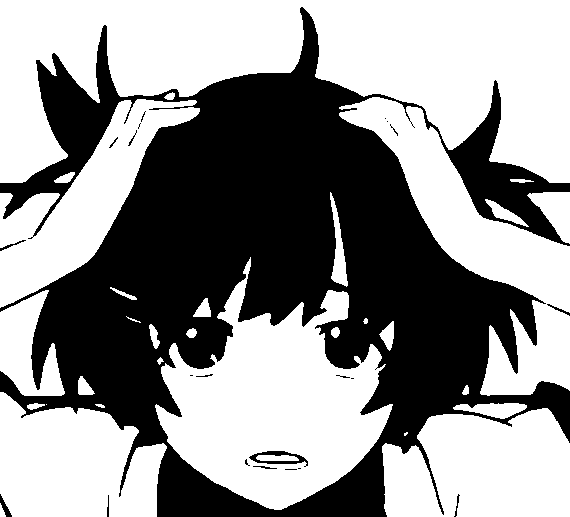
\includegraphics[scale=0.25]{hanekawa_binary}
      \caption{An image binarized with Otsu's binarization.}
    \end{figure}
  \end{exampleblock}
\end{columns}
\end{frame}

\begin{frame}
\frametitle{Cost Function}
\framesubtitle{}
\begin{itemize}[<+->]
    \item How should we measure the effectiveness?
    \item Well, we're splitting the pixels into two groups.
      Minimize the variance of each group, weighted by the
      size of the group (to minimize the expected variance).
    \item This is identical to \( k \)-means with \( k = 2 \).
    \item  However, the standard \( k \)-means algorithm is suboptimal and
      may take longer than we want. Can we do optimal \( k \)-means
      efficiently if we know the data is one-dimensional and \( k = 2 \)?
  \end{itemize}
\end{frame}

\begin{frame}
\frametitle{Otsu's Binarization, Justification}
\framesubtitle{}
\begin{itemize}[<+->]
  \item There are efficient algorithms for 1D \( k \)-means, see
    \href{https://arxiv.org/abs/1701.07204} {\textit{Fast Exact k-Means,
    k-Medians and Bregman Divergence Clustering in 1D}}.
  \item However, these algorithms are pretty complicated. 
  \item Can we make use of \( k = 2 \)?
  \item The key observation is that if we place two centers, there's only
    one point equidistant to those centers, at their midpoint. Anything to
    the left of the midpoint is assigned to one center and anything to the
    right the other.
  \item In 1D and with \( k = 2 \), we have exactly one
    \textit{threshold} value. How many possible thresholds are there?
\end{itemize}
\end{frame}

\begin{frame}
\frametitle{Otsu's Binarization, Summary}
\framesubtitle{}
\begin{itemize}
  \item Iterate over the 256 possible thresholds
  \item Maintain statistics counters 
  \item Compute the expected variance after each split 
  \item Pick the threshold with the smallest intra-class variance
\end{itemize}
\end{frame}

\subsection{Inter-class Variance}

\begin{frame}
\frametitle{Inter-class Variance}
\framesubtitle{}
Standard approach: minimizing intra-class
variance is maximizing inter-class variance.
\begin{align*}
  \shortintertext{By definition of variance,}
  \Var[\E[X \mid Y]] &= \E[(\E[X \mid Y] - \E[\E[X \mid Y]])^2] 
  \shortintertext{Using the law of total expectation,}
                     &= \E[(\E[X \mid Y] - \E[X])^2] \\ 
                     &= \sum_i P(Y = i) (\E[X \mid Y = i] - \E[X])^2 
  \shortintertext{To make the notation more concise, let the
  inter-class variance be \( \sigma_B^2 \), \( P(Y = i) \) be
  \( \omega_i \), and \( \E[X \mid Y = i] \) be \( \mu_i \):}
          \sigma_B^2 &= \omega_0 (\mu_0 - \mu)^2 + \omega_1 (\mu_1 - \mu)^2 
\end{align*}
\end{frame}

\begin{frame}
\frametitle{Inter-class Variance, Continued}
\framesubtitle{}
\begin{align*}
  \sigma_B^2 &= \omega_0 (\mu_0 - \mu)^2 + \omega_1 (\mu_1 - \mu)^2 \\
             &= \omega_0 [\mu_0^2 - 2 \mu_0 \mu + \mu^2] + \omega_1 [\mu_1^2 - 2 \mu_1 \mu + \mu^2] \\
             &= \omega_0 \mu_0^2 + \omega_1 \mu_1^2
             - 2 \mu (\omega_0 \mu_0 + \omega_1 \mu_1)
             + \mu^2 (\omega_0 + \omega_1) \\
  \shortintertext{We know \( \omega_0 + \omega_1 = 1 \)
    because they're probabilities and 
    \( \omega_0 \mu_0 + \omega_1 \mu_1 = \E[\E[X \mid Y]] = \E[X] = \mu \) so}
             &= \omega_0 \mu_0^2 + \omega_1 \mu_1^2 - \mu^2 \\
             &= \omega_0 \mu_0^2 + \omega_1 \mu_1^2 - (\omega_0 \mu_0 + \omega_1 \mu_1)^2  \\
             &= (\omega_0 - \omega_0^2) \mu_0^2 - 2 \omega_0 \omega_1 \mu_0 \mu_1 + (\omega_1 - \omega_1^2) \mu_1^2 \\
             &= \omega_0 (1 - \omega_0) \mu_0^2 - 2 \omega_0 \omega_1 \mu_0 \mu_1 + \omega_1 (1 - \omega_1) \mu_1^2 
  \shortintertext{We know \( 1 - \omega_0 = \omega_1 \)
    and likewise for \( 1 - \omega_1 \),}
             &= \omega_0 \omega_1 \mu_0^2 - 2 \omega_0 \omega_1 \mu_0 \mu_1 + \omega_0 \omega_1 \mu_1^2
              = \boxed{\omega_0 \omega_1 (\mu_0 - \mu_1)^2}
\end{align*} 
\end{frame}

\begin{frame}
\frametitle{Algorithm Overview}
\framesubtitle{}
\begin{enumerate}
  \item Precompute the number of pixels of each intensity
  \item Iterate over possible thresholds, maintaining counters
  \item Compute threshold which maximizes inter-class variance
  \item Binarize image with optimal threshold
\end{enumerate}
\end{frame}

\begin{frame}[fragile]
\frametitle{Image distribution}
\framesubtitle{}
\begin{minted}[label=frequency counts of each pixel]{python}
def histogram(img: np.array) -> np.array:
    """ Computes the distribution of the image. """
    p = np.zeros(256, dtype=np.int)
    for x in img.flatten():
        p[x] += 1
    return p
\end{minted}
\end{frame}

\begin{frame}
\frametitle{Algorithm Details}
\framesubtitle{}
\begin{itemize}
  \item We need to keep track of \( \omega_0 \) and \( \mu_0 \)
  \item Can compute \( \omega_1 \) and \( \mu_1 \) by subtraction 
  \item Easier if they are not fractions but integer counts, i.e.
    \( W_0 = |S_0| = |X| \omega_0 \) and \\
    \( A_0 = \sum_{x \mid S(x) = 0} x = |S_0| \mu_0 \) 
  \item We know we're scanning in terms of increasing threshold \( t \)
  \item So the only change is going to be pixels with intensity \( t \)
  \item Then the update is just \( W_0 + p[t] \) and \( A_0 + t \, p[t] \)
  \item \( \omega_0 = \frac{W_0}{|X|} \) and \( \mu_0 = \frac{A_0}{W_0} \)
\end{itemize}
\end{frame}

\begin{frame}[fragile]
\frametitle{}
\framesubtitle{}
\begin{algorithm}[H]
  \caption{Otsu's binarization with inter-class variance}
  \begin{minted}[frame=none,fontsize=\small]{python}
def otsu(img: np.array) -> np.array:
    """ Applies Otsu's binarization to the image. """
    h, n = histogram(img)
    X0, X1, p = 0, img.sum(), 0
    threshold, best = -1, 0
    for t in range(256):
        u1, u0 = t*h[t], h[t]
        X0, X1, p = X0 + u1, X1 - u1, p + u0
        if p > 0 and n - p > 0:
            # divide by n^2 to get the true variance
            var = p*(n - p)*(X0/p - X1/(n - p))**2
            if var > best:
                threshold, best = t, var
    return __threshold(img, threshold)
  \end{minted}
\end{algorithm}
\end{frame}

\begin{frame}[fragile]
\frametitle{Binarization}
\framesubtitle{}
Otsu's binarization computes the optimal threshold.

We want a binary image.

\begin{minted}[label=thresholding]{python}
def __threshold(img: np.array, t: int) -> np.array:
    """ Binarizes an image given a threshold. """
    return 255*(img > t)
\end{minted}

Whether it's \( > \) or \( \geq \) is arbitrary, just needs to be consistent.
\end{frame}

\subsection{Intra-class Variance}

\begin{frame}
\frametitle{Intra-class Variance}
\framesubtitle{}
\begin{itemize}
  \item We just spent a lot of time deriving inter-class variance.
  \item We needed to use the law of total variance to show
    that it's the same as minimizing intra-class variance.
  \item Why not just directly attack intra-class variance?
\end{itemize}
\begin{align*}
  \shortintertext{By the definition of expectation,}
  \E[\Var[X \mid Y]] &= \sum_i P(Y = i) \Var[X \mid Y = i]
  \shortintertext{As usual, let the intra-class variance
    be \( \sigma_W^2 \), \( P(Y = i) \) be \( \omega_i \),
  and \( \Var[X \mid Y = i] \) be \( \sigma_i^2 \):}
          \sigma_W^2 &= \omega_0 \sigma_0^2 + \omega_1 \sigma_1^2 
\end{align*}
\end{frame}

\begin{frame}
\frametitle{Intra-class Variance, Continued}
\framesubtitle{}
\begin{align*}
  \shortintertext{Now let's re-write the conditional variances using
  \( \Var[X \mid Y] = \E[X^2 \mid Y] - \E[X \mid Y]^2 \):}
  \sigma_W^2 &= \omega_0 \sigma_0^2 + \omega_1 \sigma_1^2 \\
              &= \omega_0 [\frac{\sum_{x \mid S(x) = 0} x^2}{|S_0|} - 
                          (\frac{\sum_{x \mid S(x) = 0} x}{|S_0|})^2] \\
              &+ \omega_1 [\frac{\sum_{x \mid S(x) = 1} x^2}{|S_1|} - 
                          (\frac{\sum_{x \mid S(x) = 1} x}{|S_1|})^2]
  \shortintertext{To make the notation more concise, \newline 
    let \( W_i = |S_i| \) and \( \sum x^k_i = \sum_{x \mid S(x) = i} x^k \):}
              &= \frac{W_0}{|X|} [\frac{\sum x_0^2}{W_0} - (\frac{\sum x_0}{W_0})^2] +
                 \frac{W_1}{|X|} [\frac{\sum x_1^2}{W_1} - (\frac{\sum x_1}{W_1})^2]
\end{align*} 
\end{frame}

\begin{frame}
\frametitle{Intra-class Variance, Continued}
\framesubtitle{}
\begin{align*}
  \sigma_W^2 &= \frac{W_0}{|X|} [\frac{\sum x_0^2}{W_0} - (\frac{\sum x_0}{W_0})^2] +
                \frac{W_1}{|X|} [\frac{\sum x_1^2}{W_1} - (\frac{\sum x_1}{W_1})^2] \\
             &= \frac{1}{|X|} ([\sum x_0^2 - \frac{(\sum x_0)^2}{W_0}] +
                               [\sum x_1^2 - \frac{(\sum x_1)^2}{W_1}])
  \shortintertext{Multiplying by \( |X| \) and re-arranging,}
             &= [\sum x_0^2 + \sum x_1^2] -
                [\frac{(\sum x_0)^2}{W_0} + \frac{(\sum x_1)^2}{W_1}]
\shortintertext{The first term is just the sum of squares for each \( x
\in X \), which is a constant, and we can negate the second term, swapping
the objective. Finally, putting in terms of the counter variables:}
             &= \frac{(\sum x_0)^2}{W_0} + \frac{(\sum x_1)^2}{W_1}
              = \boxed{\frac{A_0^2}{W_0} + \frac{A_1^2}{|X| - W_0}}
\end{align*}
\end{frame}

\begin{frame}[fragile]
\frametitle{}
\framesubtitle{}
\begin{algorithm}[H]
  \caption{Otsu's binarization with intra-class variance}
  \begin{minted}[frame=none,fontsize=\small]{python}
def otsu(img: np.array) -> np.array:
    """ Applies Otsu's binarization to the image. """
    h, n = histogram(img)
    X0, X1, p = 0, img.sum(), 0
    threshold, best = -1, X1*X1/n
    for t in range(256):
        u1, u0 = t*h[t], h[t]
        X0, X1, p = X0 + u1, X1 - u1, p + u0
        if p > 0 and n - p > 0:
            # for true intra-class variance
            # divide by -n then add E[X^2] 
            var = X0*X0/p + X1*X1/(n - p)
            if var > best:
                threshold, best = t, var
    return __threshold(img, threshold)
  \end{minted}
\end{algorithm}
\end{frame}

\begin{frame}
\frametitle{Commentary}
\framesubtitle{}
\begin{itemize}
  \item Both approaches are \( O(n) \) (assuming fixed 8-bit color) 
  \item Both approaches generate identical thresholds (and images)
  \item However, intra-class variance is simpler and easier to derive
  \item It's also easier to convert to pure integer arithmetic,
    by storing fractions as numerator/denominator
\end{itemize}
\end{frame}

\subsection{Conclusion}

\begin{frame}
\frametitle{Example}
\framesubtitle{Otsu's binarization ran on an image}
\begin{figure}[h!]
    \centering
    \begin{subfigure}[h]{0.49 \textwidth}
      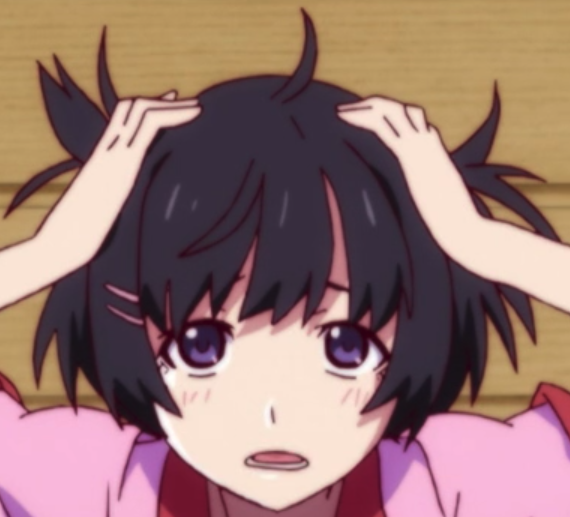
\includegraphics[scale=0.23]{hanekawa}
      \caption{The original image.}
    \end{subfigure}
    \hfill
    \begin{subfigure}[h]{0.49 \textwidth}
      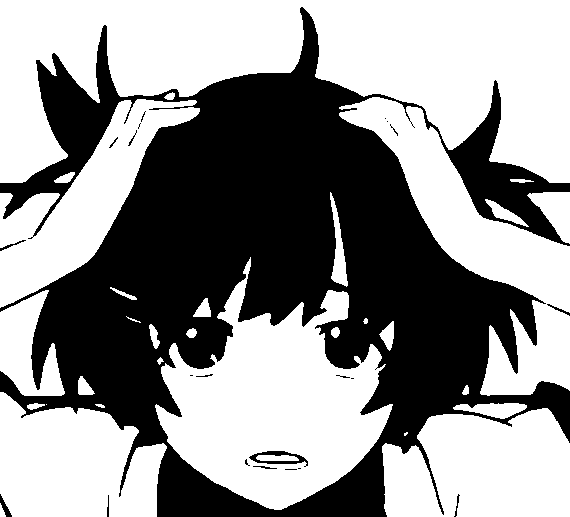
\includegraphics[scale=0.23]{hanekawa_binary}
      \caption{After Otsu's binarization.}
    \end{subfigure}
    \caption{Before and after Otsu's binarization.}
\end{figure}
\end{frame}

\begin{frame}
\frametitle{Histogram and Inter-class Variance over Thresholds}
\framesubtitle{}
\begin{figure}[h!]
  \centering
  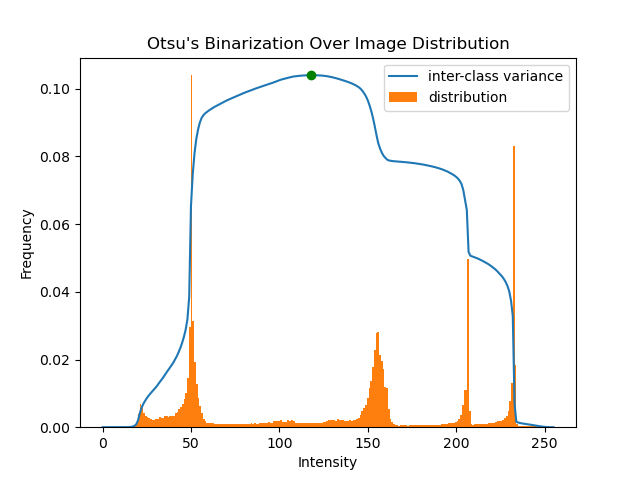
\includegraphics[scale=0.50]{histogram}
  \caption{Inter-class variance over increasing threshold value.}
\end{figure}
\end{frame}

\begin{frame}
\frametitle{Last Comments}
\framesubtitle{}
\begin{itemize}
  \item The image might have noise. Reduce noise with
    a Gaussian kernel, averaging, or other techniques.
  \item We've been using 8 bits per color channel for a pretty long time.
    But there's no reason why images with 16-bit color or even 48-bit
    color won't catch on. In that case Otsu's takes \( O(N 2^b) \)
    where \( b \) is the number of bits per channel, which will not
    scale with increasing color depth.
  \item People may need to quantize their images or apply a
    sophisticated 1D \( k \)-means algorithm, optimized for \( k = 2 \).
\end{itemize}
\end{frame}

\section{References}

\begin{frame}
\frametitle{References}
\framesubtitle{}
\begin{enumerate}
  \item \href{https://github.com/pwhitetj/probtheory}
    {Dr. White's probability theory textbook}
  \item My lectures on
    \begin{itemize}
      \item \href{https://stephen-huan.github.io/assets/pdfs/cs-lectures/math/probability-theory/gacha-optimization/writeup.pdf\#page=4}
        {Probability theory}
      \item \href{https://stephen-huan.github.io/assets/pdfs/cs-lectures/computer-vision/kmeans-kd-tree/handout.pdf}
        {\( k \)-means}
    \end{itemize}
  \item Wikipedia articles on 
    \begin{itemize}
      \item \href{https://en.wikipedia.org/wiki/Probability_axioms}
        {Probability axioms}
      \item \href{https://en.wikipedia.org/wiki/Law_of_total_probability}
        {Law of total probability}
      \item \href{https://en.wikipedia.org/wiki/Law_of_total_expectation}
        {Law of total expectation}
      \item \href{https://en.wikipedia.org/wiki/Law_of_total_variance}
        {Law of total variance}
      \item \href{https://en.wikipedia.org/wiki/K-means_clustering}
        {\( k \)-means}
      \item \href{https://en.wikipedia.org/wiki/Otsu\%27s_method}
        {Otsu's method}
    \end{itemize}
  \item \href{http://www.labbookpages.co.uk/software/imgProc/otsuThreshold.html}
    {Otsu Thresholding}
  \item \href{https://docs.opencv.org/master/d7/d4d/tutorial_py_thresholding.html}
    {OpenCV documentation}
\end{enumerate}
\end{frame}

% \printbibliography
\end{document}
